\externaldocument[-f]{c2_foundations}
\chapter{Experimental Setup}

This chapter presents the methodology used in this thesis. First, it is explained how different frameworks introduced in \cref{chap:2} are put into use. Then, the algorithms used in data generation and inference are given in detail. The results from these experiments are presented in the succeeding chapter.

\section{The Model}
\begin{wrapfigure}{r}{3cm}
	\begin{center}
		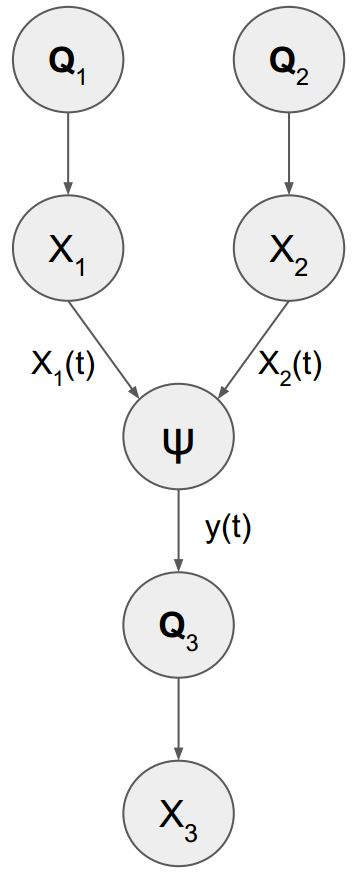
\includegraphics[width=2.5cm]{figures/h_model}
		\caption{Hierarchical model.}
	\end{center}
	\label{fig:h_model}
\end{wrapfigure} 
A detailed graphical model explored in this thesis is given in the \cref{fig:h_model}. This model presents an intersection of continuous-time Bayesian network and partially observable Markov decision process frameworks. 
\begin{itemize}
	\item The transition models of the nodes $ X_1, X_2$ and $ X_3 $, and the dependencies between them are modelled as CTBN.
	\item The interaction of agent node $ X_3 $ and its environment is modelled as POMDP.
\end{itemize}

\subsection{CTBN Model}

The transition models of the nodes and the dependencies between them are modelled as continuous-time Bayesian network (CTBN), denoted by \textbf{X}. The network \textbf{X} represents a stohastic process over a structured multivariate state space $ \rchi = [\rchi_1, \rchi_2, \rchi_3] $. 

The parent nodes $X_{1}$ and $ X_{2} $ emit their states as messages. The dynamics  of these nodes are modelled as independent homogeneous continuous-time Markov processes $X_{i}(t)$, with binary-valued states $ \rchi_{i} = \left\lbrace 0, 1 \right\rbrace  $ for $ i \in \left\lbrace 1,2 \right\rbrace $. These processes are defined by transition intensity matrices $ \textbf{Q}_{i} $, which are assumed to be Gamma distributed with shape and rate parameters $ \boldsymbol{\alpha} = [\alpha_0, \alpha_1] $ and $ \boldsymbol{\beta} = [\beta_0, \beta_1] $, respectively, and are in the following forms.
\begin{align}
\textbf{Q}_i &= 
\begin{bmatrix}
-q^i_{0} & q^i_{0} \\
q^i_{1} &  -q^i_{1}
\end{bmatrix}
\label{eq:Q_parents}\\
\textbf{Q}_{i} &\sim Gam(\boldsymbol{\alpha}^i, \boldsymbol{\beta}^i)\ \ for\ i \in \left\lbrace 1,2\right\rbrace \label{eq:gamma_priors}
\end{align}
It should be noted that in \autoref{eq:Q_parents}, the suffixes are simplified using the fact that $ q_{i} = \sum_{i \neq j} q_{i,j}$.

The agent  $ X_{3} $ is modelled as inhomogenouos continuous-time Markov process with binary states $ \rchi_{3} = \left\lbrace 0, 1 \right\rbrace  $ and set of actions $ a \in \left\lbrace a_0, a_1\right\rbrace  $, and set of transition intensity matrices which contains one matrix corresponding to each action, $ \textbf{\textit{Q}}_{3 \mid a} = \left\lbrace \textbf{Q}_{3\mid a_{0}}, \textbf{Q}_{3\mid a_{1}} \right\rbrace $.
%\begin{equation}
%\textbf{Q}_{a_k} \sim Gam(\alpha_{a_k}, \beta_{a_k})
%\end{equation}

The dependencies are represented by set of parents for each node $ \textbf{U}_{n} = Par(X_n) $ and for the model shown in \cref{fig:h_model} can be written as follows:
\begin{align*}
\textbf{U}_{1}, \textbf{U}_{2} & = \emptyset \\
\textbf{U}_{3} & = \left\lbrace X_1, X_2 \right\rbrace 
\end{align*}

\subsection{POMDP Model}
In a conventional POMDP scenario, there are two problems to be addressed, one is belief state update and the other is policy optimization. As mentioned in \cref{sec:belief_POMDP}, in the problem at hand, the policy of agent $ X_3 $ is assumed to be optimal and given. Thus, the POMDP model of the agent only consists of belief state update. A detailed view of the agents interaction with its environment from POMDP framework perspective is given in the \cref{fig:POMDP_pers}. \\
\begin{figure}[htb]
	\begin{center}
		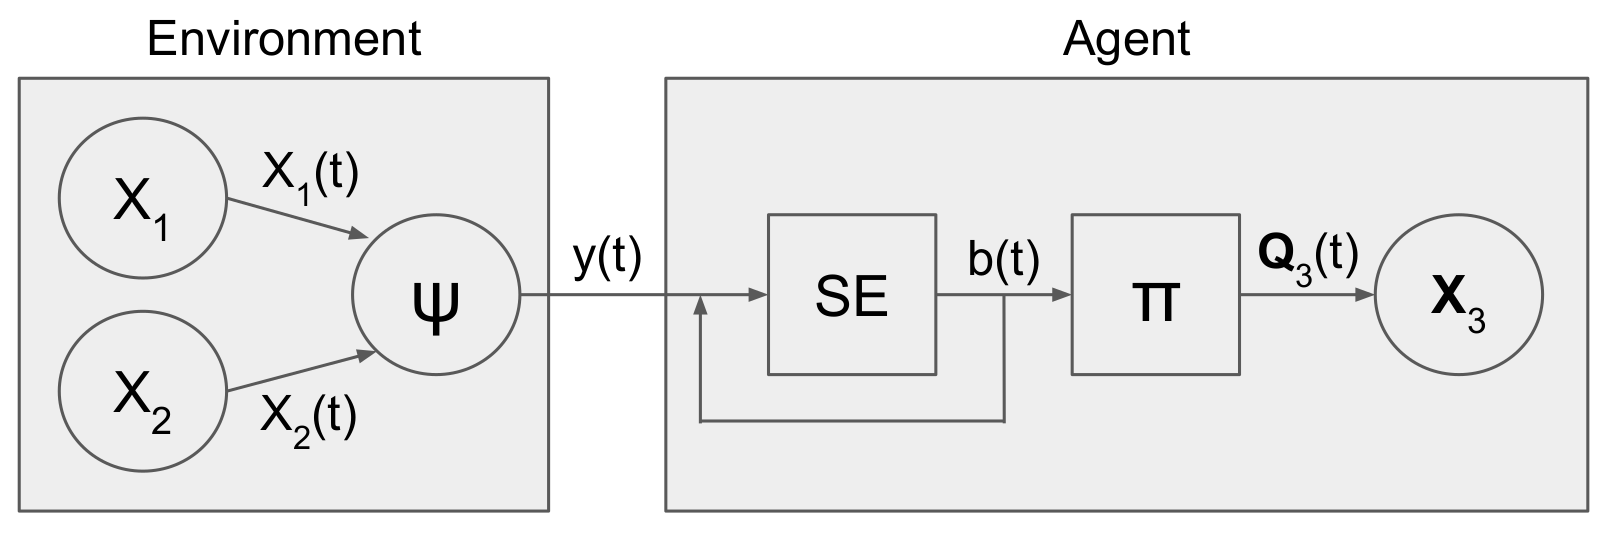
\includegraphics[width=.75\textwidth]{figures/POMDP_graph}
		\caption{Closer look to agent-environment interaction from the perspective of POMDP framework.}
		\label{fig:POMDP_pers}
	\end{center}
\end{figure}\\
It should be noted that, the interaction in \cref{fig:POMDP_pers} is only one-sided, the state or action of the agent does not affect the environment.
\subsubsection{Observation Model}
The messages sent by the parent nodes are translated by the observation model. The agent node $ X_3 $ does not have a direct access to the messages, but observes a translation of them. The observation model gives a probability distribution over the observation for each combination of parent messages.
\begin{equation}
\psi(x_1, x_2) = \operatorname{Pr}(y(t) \mid X_{1}(t), X_{2}(t))
\end{equation}

\subsubsection{Belief State}
The \textit{state estimator} (labelled as SE in \cref{fig:POMDP_pers}) forms a belief over the parent states, denoted by $  b(x_{1}, x_{2}; t) $. 
\begin{equation}
b(x_{1}, x_{2}; t) = \operatorname{Pr}( X_{1}(t) = x_{1},  X_{2}(t) = x_{2}\mid y_{1}, ..., y_{t})
\end{equation}
\paragraph*{Exact Belief State Update}
\label{par:bs_exact}
Given the transition intensity matrices of parent nodes, $ \textbf{Q}_1 $ and $ \textbf{Q}_2 $, the continuous-time belief state update poses a filtering problem for CTMPs (\cref{sec:filtering_CTMC}). 

Consider a subsystem of CTBN model, consisting of only the parent nodes, $ X_1 $ and $ X_2 $. These two processes can be represented as one single \textit{joint} process, $ X_P $, with multivariate state space $ \rchi_{P} = \left\lbrace (x_1, x_2)\right\rbrace_{x_1\in \rchi_1, x_2 \in \rchi_2}  = \left\lbrace (0,0), (0,1), (1,0), (1,1)\right\rbrace  $. The transition intensity matrix of the new joint system, $ \textbf{Q}_P $ is obtained by amalgamation operation between $ \textbf{Q}_{1} $ and  $ \textbf{Q}_{2} $ (see \cref{ap:amalgamation}) \cite{Nodelman1995}.
\begin{equation}
\textbf{Q}_P = \textbf{Q}_{1} * \textbf{Q}_{2}
\end{equation}
Then, the filtering problem can be formulated according to this joint process of parents.
\begin{equation}
b(x_p; t) = \operatorname{Pr}( X_P(t) = x_{p} \mid y_{1}, ..., y_{t})
\end{equation}
Consider discrete-time observations from this process, denoted by $ y_{1}=y(t_{1}), ..., y_{N}=y(t_{N}) $ and time-dependent belief state $ b(t) $ as a row vector with $ \left\lbrace b(x_p;t)\right\rbrace_{x_p \in \rchi_P} $. Following \autoref{eq:b_cont} and \autoref{eq:b_jump}, the belief state update is evaluated as
\begin{equation}
b(t) = b(0) \exp(t\textbf{Q}_P)
\end{equation}
with the initial condition $ b(0) $.
The update at discrete times of observation $ y_{t} $ is
\begin{align}
b(x_p; t_{N}) &= Z_{N}^{-1}\ {\operatorname{Pr}(y_{N} \mid X_P(t_{N})=x_p)}\ {b(x_p; t_{N}^{-})} \\ & = Z_{N}^{-1}\ \psi(x_p) \ {b(x_p; t_{N}^{-})}
\end{align}
where $ Z_{N} = \sum_{x_p\in \rchi_P} \psi(x_p)\ b(x_p; t_{N}^{-}) $ is the normalization factor.

\paragraph*{Belief State Update Using Particle Filter}
\label{par:bs_partFilt}
The assumption that full information of parent dynamics being available is unrealistic. In an environment as described above, the agent most probably doesn't have access to the parameters $ \textbf{Q}_1 $ and $ \textbf{Q}_2 $, rather may have some prior beliefs over them. Thus, in order to simulate a more realistic model and be able to marginalize out these parameters from inference problem, the joint process (introduced in previous section) is replaced with its marginalized counterpart. Using the Gamma-priors over $ \textbf{Q}_1 $ and $ \textbf{Q}_2 $ (\autoref{eq:gamma_priors}) and sufficient statistics over the particle history, the particles are drawn from this marginalized process. With every new observation, the particles are propogated through the process, while the sufficient statistics are updated and the parameters are re-estimated after each particle using the \autoref{eq:estimated_Q}. The belief state then obtained as the distribution of states over the particles,
\begin{equation}
b(x_p; t) = \frac{1}{N} \sum_{i=1}^{N} \delta_{p_i(t), x_p}
\end{equation}
where $ N $ is the number of particles, $ \textbf{p} $ is the set of particles, and $\delta$ is the Kronecker delta.

\begin{algorithm}[H]
	\SetKwInOut{KwIn}{Input}
	\SetKwInOut{KwOut}{Output}
	\KwIn{Observation $ y_{k} $ at time $ t_{k} $, set of particles $\textbf{p}^{k-1} $, estimated $ \hat{Q} $}
	\KwOut{New set of particles $ \textbf{p}^{k} $, $ \textbf{b}^{[t_{k-1}, t_{k}]} $}
	
	\vspace{+4pt}
	\begin{algorithmic}[1]
		\FOR{$p_{m} \in \textbf{p}^{k-1}$}
		\STATE {$p_{m} = \left\lbrace x_{m}, \hat{Q}\right\rbrace \leftarrow Propagate\ particle\ through\ marginal\ process\ from\ t_{k-1}\ to\ t_{k}$ }\\
		
		\STATE {$\hat{Q} \leftarrow sufficient\ statistics\ added\ from\  p_{m}[t_{k-1}, t_{k}]$} \\
		\tcp*[h] {observation likelihood assigned as particle weight}
		\STATE{$w_{m} \leftarrow p(y_{k} \mid X_P(t_{k})=x_{m}) $} 
		\ENDFOR \\
		\tcp*[h]{belief state from $ t_{k-1} $ to $ t_{k} $}
		\STATE{$ \textbf{b}^{[t_{k-1}, t_{k}]} \leftarrow \left\lbrace \frac{1}{N} \sum_{i=1}^{N} \delta_{p_i^{[t_{k-1}, t_{k}]} , x_p}\right\rbrace_{x_p \in \rchi_P} $}\\
		\tcp*[h]{normalize weights}
		\STATE{$ w_{m} \leftarrow \frac{w_{m}}{\sum_{m} w_{m}}$   }\\
		\tcp*[h]{  resample particles}
		\FOR{$ p_{m} \in \textbf{p}_{k} $} 
		\STATE{$ p_{m} \leftarrow Sample\ from\ p_{k}\ with\ probabilities\ w_{m}\ with\ replacement$}
		\ENDFOR 
	\end{algorithmic}
	\caption{Marginal particle filter for belief state update}
\end{algorithm}

\subsubsection{Optimal Policy}

The optimal policy is defined using a polynomial function of belief state.
\begin{equation}
\pi(b) = 
\begin{cases}
a_0 & \quad \text{if } \textbf{w}b^\intercal > 0.5 \\
a_1 & \quad \text{otherwise}
\end{cases}
\end{equation}
where \textbf{w} is a row vector of weights.

Given the optimal policy, $ \pi(b) $, the agent takes an action based on the belief state. In the setting described above, taking an action means to change its internal dynamics to the transition intensity matrix corresponding to that action.
\begin{align}
a(t) &= \pi(b(t))\\
\textbf{Q}_3(t) & = \begin{cases}
\textbf{Q}_{3\mid a_{0}} & \quad \text{if } a(t) = a_0 \\
\textbf{Q}_{3\mid a_{1}} & \quad \text{otherwise}
\end{cases}
\end{align}

\section{Inference of Observation Model}
Inference problem is considered for deterministic observation models. Considering the number of states of parents and the observations, there are a number of possible observation models. Given the parent trajectories, the belief state and the resulting $ \textbf{Q}_3 $ trajectory is computed for each observation model. Then the likelihood of $ X_3 $ trajectory given these  $ \textbf{Q}_3 $  trajectories are compared for maximum likelihood estimation.
%TODO correct this
\begin{equation}
\hat{\psi} = argmax \operatorname{Pr}(X_3^{[0,T]} \mid Q_3^{[0,T]})
\end{equation}

\textbf{QUESTION: Is this okay to put results for 3 observation models or should i run the results for all 81 observation models we have? The problem is there are some observation models that we wouldn't be able to distinguish}
\subsection{Likelihood Model}
Consider a trajectory in the dataset, denoted by $ \textbf{X}^{[0,T]} = \left\lbrace X_1^{[0,T]} , X_2^{[0,T]}, X_3^{[0,T]}\right\rbrace $. The set of parameters to the system, as introduced before, is written as $  \theta = \left\lbrace  \textbf{Q}_{1}, \textbf{Q}_{2}, \pi, \psi \right\rbrace $. Then likelihood of the sample trajectory $ \textbf{X}^{[0,T]} $ can be written as:
\begin{align}
P(\textbf{X}^{[0,T]} \mid \theta ) & = P(X_{1}^{[0, T]}, X_{2}^{[0, T]}, X_{3}^{[0, T]} \mid \textbf{Q}_{1}, \textbf{Q}_{2}, \pi, \psi) \nonumber\\
& = P(X_{3}^{[0, T]} \mid X_{1}^{[0, T]}, X_{2}^{[0, T]}, \textbf{Q}_{1}, \textbf{Q}_{2}, \pi, \psi) \ P(X_{1}^{[0, T]}\mid \textbf{Q}_{1}) \ P(X_{2}^{[0, T]}\mid \textbf{Q}_{2}) \nonumber\\ & = P(X_{3}^{[0, T]} \mid X_{1}^{[0, T]}, X_{2}^{[0, T]}, \pi, \psi) \ P(X_{1}^{[0, T]}\mid \textbf{Q}_{1}) \ P(X_{2}^{[0, T]}\mid \textbf{Q}_{2}) \nonumber\\ & = P(X_{3}^{[0, T]}\mid \textbf{Q}_{3}^{[0, T]}) \ P(X_{1}^{[0, T]}\mid \textbf{Q}_{1}) \ P(X_{2}^{[0, T]}\mid \textbf{Q}_{2}) 
\label{eq:system_llh}
\end{align}
As mentioned before, it is plausible to marginalize out the parameters $ \textbf{Q}_1 $ and $ \textbf{Q}_2 $, for a more realistic model and inference. Noting that in case the belief state is updated using filtering of CTMPs (See \cref{par:bs_exact}), $ \textbf{Q}_{3}^{[0, T]} $ becomes a deterministic function of all the parameters including $ \textbf{Q}_1 $ and $ \textbf{Q}_2 $, the marginalization cannot be carried out analytically on \autoref{eq:system_llh}. On the other hand, particle filtering removes this dependency on $ \textbf{Q}_1 $ and $ \textbf{Q}_2 $ by using marginalized counterpart of CTMPs (See \cref{par:bs_partFilt}), leaving it straightforward to marginalize out the parameters on \autoref{eq:system_llh}.

Marginalizing the likelihood over $ Q_{1} $ and $ Q_{2} $:
\begin{align}
P(\textbf{X}^{[0,T]} \mid \pi, \psi ) & = 	\int \int P(\textbf{X}^{[0,T]} \mid \theta ) \ P(\textbf{Q}_{1}) \ P(\textbf{Q}_{2}) \ d\textbf{Q}_{1}d\textbf{Q}_{2} \nonumber\\ 
& = \int \int P(X_{3}^{[0, T]}\mid \textbf{Q}_{3}^{[0, T]}) \ P(X_{1}^{[0, T]}\mid \textbf{Q}_{1}) \ P(X_{2}^{[0, T]}\mid \textbf{Q}_{2}) \ P(\textbf{Q}_{1}) \ P(\textbf{Q}_{2})\ d\textbf{Q}_{1}d\textbf{Q}_{2} \nonumber\\ 
& = P(X_{3}^{[0, T]}\mid \textbf{Q}_{3}^{[0, T]}) \int  P(X_{1}^{[0, T]}\mid \textbf{Q}_{1}) \ P(\textbf{Q}_{1}) \ d\textbf{Q}_{1} \int P(X_{2}^{[0, T]}\mid \textbf{Q}_{2})\ P(\textbf{Q}_{2})\ d\textbf{Q}_{2}
\label{eq:Marg_llh}
\end{align}
Marginalized likelihood function for binary-valued homogenous CTMP is derived in \autoref{ap:marg_llh_ctmp}.

Plugging \autoref{eq:Marg_traj} in \autoref{eq:Marg_llh} for both $ X_{1} $ and $ X_{2} $:
\begin{align}
\begin{split}
P(\textbf{X}^{[0,T]} \mid \pi, \Phi ) = P(X_{3}^{[0, T]}\mid Q_{3}^{[0, T]}) \prod_{x_{1}\in{0,1}} \frac{\beta_{x_{1}}^{\alpha_{x_{1}}}}{\Gamma(\alpha_{x_{1}})} \ (T_{x_{1}}+\beta_{x_{1}})^{M_{x_{1}} + \alpha_{x_{1}}}\ \Gamma(M_{x_{1}} + \alpha_{x_{1}})  \\  \prod_{x_{2}\in{0,1}} \frac{\beta_{x_{2}}^{\alpha_{x_{2}}}}{\Gamma(\alpha_{x_{2}})} \ (T_{x_{2}}+\beta_{x_{2}})^{M_{x_{2}} + \alpha_{x_{2}}}\ \Gamma(M_{x_{2}} + \alpha_{x_{2}})
\label{eq:Marg_llh_final}
\end{split}
\end{align}

\section{Data Generation}
The dataset contains a number of trajectories drawn from CTBN \textbf{X}. Following the notation in \cref{chap:2}, K trajectories in time interval $ [0, T] $ are denoted by $ \xi_T = \left\lbrace \textbf{X}^{[0,T], 1}, \textbf{X}^{[0,T], 2}, ..., \textbf{X}^{[0,T], K} \right\rbrace  $, where $ \textbf{X}^{[0,T],k} = \left\lbrace X_1^{[0,T],k} , X_2^{[0,T],k}, X_3^{[0,T],k}\right\rbrace $ denotes a single trajectory for all nodes. Every trajectory comprises of state transitions in the interval, and the times of these transitions. 

\subsection{Sampling Algorithm}
In order to sample trajectories from CTBN, two sampling algortihms introduced in \cref{sec:sampling_alg} are combined. Gillespie algorithm is used to sample from the parent nodes, $ X_1 $ and $ X_2 $, while thinning algorithm is applied to overcome the challenges that come with conditional intensity matrix of the agent, $ X_3 $. It should be noted that, \cref{alg:generative_ctbn} is applicable to any nodes in a CTBN, both homogenous and conditional MPs. However, since in this setting, the intensity matrix is conditioned on the belief state and the policy, instead of directly on the parent states, a more general algorithm suitable for inhomogenous MPs, thinning algorithm, is preferred. \cref{alg:sampling} describes the procedure to draw samples using particle filtering. 

\begin{algorithm}[H]
	\SetKwInOut{KwIn}{Input}
	\SetKwInOut{KwOut}{Output}
	\SetKwInOut{Init}{Initialize}
	
	\KwIn{Gamma-prior parameters on parents' transition intensity matrices $ \alpha^1, \beta^1, \alpha^2, \beta^2 $\\
		Set of agent's transition intensity matrices $ \textbf{\textit{Q}}_3 $\\
		$ T_{max} $ to terminate simulation}
	\KwOut{Sample trajectory of the network}
	\Init{Sample $ \textbf{Q}_1 $ and $ \textbf{Q}_2 $ from their priors\\ 
		Initialize nodes uniformly $ X_{n}(0) = x_{i} \in \rchi_n$ \\
		Initialize particles uniformly $ p^i(0) = x_{p} \in \rchi_P$\\
		$ t=0 $}
	
	\begin{algorithmic}[1]
		\WHILE{$ t < T_{max} $}
		\STATE{Draw next transition for $ X_1 $ and $ X_2 $ ($ \tau_{parent}$, $ x_1 $ and $ x_2 $ using \cref{alg:generative_ctbn})}
		\STATE{$ t_{parent} \leftarrow t + \tau_{parent} $}	\tcp*[h]{transition time for parents} 
		\STATE{$ y_{t_{parent}} \sim \psi(x_1, x_2)$} \tcp*[h]{new observation at $ t_{parent} $}
		\STATE{Update particle filter and obtain $ \textbf{b}^{[t, t_{parent}]} $}
		\STATE{$ a^{[t, t_{parent}]} \leftarrow \pi(\textbf{b}^{[t, t_{parent}]}) $}
		\STATE{$ \textbf{Q}_3^{[t, t_{parent}]} \leftarrow \textbf{Q}_{3\mid a^{[t, t_{parent}]}} $}
		\STATE{$ t_{agent} \leftarrow t$}
		\WHILE{$ t_{agent} < t_{parent} $}
		\STATE{\text{the upper bound for intensity,} $ q_3^{*}$} \footnotemark
		\STATE{\text{transition time $ \tau_{agent} $ drawn by }  $ u \sim U(0, 1)$ \text{ and } $ \tau_{agent} = \frac{-ln(u)}{q_3^{*}} $}
		\STATE{$ t_{agent} \leftarrow t_{agent} + \tau_{agent} $}
		\STATE{\text{draw } $s \sim U(0, 1)$, \text{accept transition if} $ s \leq \frac{q_3(t_{agent})}{q_3^{*}}$}
		\ENDWHILE
		\STATE{$ t \leftarrow t_{parent} $}
		\ENDWHILE
	\end{algorithmic}
	\caption{Sampling trajectories with particle filtering}
	\label{alg:sampling}
\end{algorithm}
\footnotetext{q is the transition intensity associated with the current state of the agent.}

\section{Configurations}
The configurations given below are used for the results presented in the following chapter, if not specified otherwise.
\begin{itemize}
	\item Gamma priors for parent dynamics such that $ \textbf{Q}_{i} \sim Gam(\boldsymbol{\alpha}^i, \boldsymbol{\beta}^i)$ for $i \in \left\lbrace 1,2\right\rbrace $, and $ \boldsymbol{\alpha} = [\alpha_0, \alpha_1] $ and $ \boldsymbol{\beta} = [\beta_0, \beta_1] $
	\begin{align}
		\boldsymbol{\alpha}^1 = [5,10] &, \boldsymbol{\beta}^1 = [5,20] \\
		\boldsymbol{\alpha}^2 = [20,20] &, \boldsymbol{\beta}^2 = [20,10]
		\label{eq:gamma_params}
	\end{align}
	\item Transition intensity matrices of $ X_1 $ and $ X_2 $ sampled from priors given above
	\begin{align}
		\textbf{Q}_1 &= 
		\begin{bmatrix}
		-1.117 & 1.117 \\
		0.836 &  -0.836
		\end{bmatrix} \\
		\textbf{Q}_2 &= 
		\begin{bmatrix}
		-1.077 & 1.077 \\
		2.324 &  -2.324
		\end{bmatrix}
	\end{align}
	\item State space, $ \textit{S} = \rchi_{P} = \left\lbrace (0, 0), (0, 1), (1, 0),(1, 1)\right\rbrace $
	\item Observation space, $ \textit{O} = \left\lbrace 0, 1, 2 \right\rbrace $
	\item Action space, $ \textit{A} = \left\lbrace a_{0}, a_{1} \right\rbrace = \left\lbrace 0, 1\right\rbrace $
	\item The set of transition intensity matrices of $ X_3 $
	\begin{align}
		\textbf{\textit{Q}}_3 = \left\lbrace \textbf{Q}_{3\mid a_{0}}, \textbf{Q}_{3\mid a_{1}} \right\rbrace = \left\lbrace 
			\begin{bmatrix}
			-0.5 & 0.5 \\
			2 &  -2
			\end{bmatrix}, 
			\begin{bmatrix}
			-3 & 3 \\
			0.02 &  -0.02
			\end{bmatrix} 
			\right\rbrace 
	\end{align}
	\item Number of particles, $ N = 200 $
\end{itemize}

%\begin{table}[!htb]
%	\begin{minipage}{.5\linewidth}
%		%		\centering
%		\begin{tabular}{c c}
%			\hline 
%			\textbf{Parameter} & \textbf{Value} \\ 
%			\hline 

%			\hline 
%		\end{tabular}
%		\caption{configuration}
%	\end{minipage}%
%	\begin{minipage}{.5\linewidth}
%		%		\centering
%		\begin{tabular}{c c c}
%			\hline 
%			\textbf{Parameter} & \textbf{Value} 
%			\hline 

%			\hline 
%		\end{tabular}
%		\caption{configurations}
%	\end{minipage} 
%\end{table}
